% Internal IEEE TIP manuscript draft for the current direct semantic-pole calibration.
% Current method and reproduction details: experiments/semantic_isp/CURRENT_METHOD.json and docs/REPRODUCING.md
% Do not claim human preference, independent perceptual quality, or request generalization
% for Exp81. Verify references, authors, data rights, and add independent/user evaluation.

\documentclass[journal]{IEEEtran}
\usepackage{amsmath,amssymb}
\usepackage{booktabs}
\usepackage{tabularx}
\usepackage{graphicx}
\usepackage{cite}
\usepackage{url}

\newcommand{\CLIP}{\mathrm{CLIP}}
\newcommand{\ISP}{\mathrm{ISP}}
\newcommand{\cosim}{\operatorname{cos}}
\newcommand{\clipop}{\operatorname{clip}}

\begin{document}

\title{Semantic ISP Pole Calibration and FiveK Fit-Render Annotations}
\author{Author names and affiliations to be finalized}
\markboth{IEEE TRANSACTIONS ON IMAGE PROCESSING, DRAFT, 2026}%
{Author Names: Calibrating Semantic ISP Poles}
\maketitle

\begin{abstract}
Natural-language descriptions of appearance do not directly specify camera image-signal-processor (ISP) parameters. We study a bounded mapping from text to six bipolar semantic controls and document FiveK-ISPVA-105, a 105-scene annotation dataset of fitted ISP renders. The active Exp81 system uses OpenAI CLIP ViT-B/32, sixteen tuned descriptors per pole, descriptor-level median aggregation across seven RAW images, and direction-aligned q90 endpoint selection. The two most extreme descriptors also define each pole centroid. The resulting ISP has six global degrees of freedom, with gray/white and skin protection applied only to palette. Across 525 FiveK expert-fit pairs, the optimized in-sample display MAE decreases from 0.1233 to 0.0321; this is a training-fit statistic, not an independent quality measure. Assistant-authored D1-D4 descriptions cover all 525 fits, whereas estimated filter-style names and Instagram/app resemblance references cover only 55 fits. No human preference or open-vocabulary generalization claim is made.
\end{abstract}

\begin{IEEEkeywords}
Image signal processing, text-guided image processing, RAW imaging, vision--language models, semantic control, differentiable optimization.
\end{IEEEkeywords}

\section{Introduction}
A request such as ``warmer,'' ``muted,'' or ``retro'' describes an intended appearance rather than an ISP configuration. The effect may involve white balance, saturation, tone, contrast, detail, or palette. This work studies a text representation with signed bipolar poles and a direct mapping to six bounded physical controls.

Text-guided image processing includes learned tone-adjustment systems and direct VLM-guided optimization. CLIPtone learns text-conditioned tone adjustment \cite{lee2024cliptone}; Mayer \emph{et al.} optimize a differentiable color ISP using image--text similarity \cite{mayer2025language}. We do not claim to be the first to use language or CLIP to tune image processing. Our focus is phrase-level calibration of signed semantic poles, one-control-at-a-time physical tuning, and direction-aware endpoint selection.

The system has an offline calibration stage and a request-time projection stage. During calibration, a frozen vision--language model scores a processed RAW crop against an exact descriptor phrase while one ISP control is optimized. We independently calibrate the text centroids, score scales, relevance gate, and physical endpoints for each model. At request time, text embeddings from the selected model are compared with its positive and negative pole centroids, then mapped to bounded controls. Request-time processing does not run iterative image-side image-encoder optimization.

The contributions of this study are:
\begin{itemize}
    \item A six-axis text-to-ISP mapping with one bounded physical control per bipolar semantic axis.
    \item A joint descriptor-tail procedure that selects physical endpoints and two-phrase CLIP centroids from phrase-level RAW tuning records.
    \item A differentiable linear-RGB ISP with explicit display-referred contrast, nearest-swatch palette mapping, and palette-only gray/skin protection.
    \item FiveK-ISPVA-105: 2,100 fit descriptions, limited assistant-authored style-name and Instagram/app resemblance subsets, and a documented annotation protocol.
    \item An in-sample six-control fit-to-photographer benchmark and an auditable set of calibration and embedding-geometry diagnostics.
\end{itemize}

The results are development-stage, same-model calibration evidence. They do not establish perceptual preference, semantic generalization of the final Exp81 calibration, runtime, or camera deployment.

\section{Related Work}
CLIPtone uses learned language-conditioned components for tone adjustment \cite{lee2024cliptone}. Mayer \emph{et al.} provide a close precedent for directly optimizing a differentiable color ISP against a VLM similarity objective \cite{mayer2025language}. T2ONet maps language instructions to editing operations \cite{shi2021t2onet}. CRISP provides controllable ISP representations without a natural-language interface \cite{kimlee2024crisp}, while DynamicISP uses downstream task feedback to adapt ISP parameters \cite{yoshimura2023dynamicisp}. CLIP-IQA uses positive and negative prompts for image-attribute assessment \cite{wang2023clipiqa}. These approaches differ in control representation, training, or objective; they motivate the problem but do not validate the current system.

SigLIP uses a sigmoid-based image--text pretraining objective \cite{zhai2023siglip}. It was evaluated as a historical alternative in Exp70, but the active implementation and all new autotuning use OpenAI CLIP ViT-B/32.

\section{Method}
\subsection{Text Pole Centroids and Coordinates}
Let $k\in\{1,\ldots,6\}$ identify an axis, $s\in\{-1,+1\}$ a pole direction, and $d_{k,s,n}$ one of its sixteen descriptors. Single-control RAW autotuning yields seven physical settings $\theta^*_{k,s,n,i}$ per descriptor. Exp81 first takes the per-descriptor median and then a direction-aligned 90th percentile across the sixteen medians:
\begin{equation}
 \bar\theta_{k,s,n}=\operatorname{median}_{i=1,\ldots,7}\theta^*_{k,s,n,i},\quad
 z_{k,s,n}=s(\bar\theta_{k,s,n}-\theta_{0,k}),\\
 \theta_{k,s}=\theta_{0,k}+s\max\!\left(0,Q_{0.9}\!\left(\{z_{k,s,n}\}_{n=1}^{16}\right)\right).
\end{equation}
Positive poles use the numerical q90 and negative poles the numerical q10 of the descriptor medians; unsupported directions fall back to neutral. The same directional ranking selects the two most extreme descriptors for the centroid:
\begin{equation}
 \mathbf{c}_{k,s}=\operatorname{norm}\!\left(\sum_{n\in S_{k,s}}
 \operatorname{norm}(f_T(d_{k,s,n}))\right),\quad
 S_{k,s}=\operatorname{Top2}_{n}(z_{k,s,n}).
\end{equation}
The two selected embeddings are individually L2-normalized, averaged, then normalized again. The generic-photo score origin, sign-specific scales, and relevance gate are recalibrated from these selected centroids. For a normalized query embedding $\mathbf{z}_q$,
\begin{equation}
 r_k(q)=\mathbf{z}_q^\top\mathbf{c}_{k,+}-\mathbf{z}_q^\top\mathbf{c}_{k,-},\quad
 x_k=0.4\,g_k(q)\,\operatorname{clip}\!\left(\frac{r_k(q)-o_k}{a_{k,\operatorname{sign}(r_k-o_k)}},-1,1\right),
\end{equation}
where $o_k$ is the score origin, $a_{k,+}$ and $a_{k,-}$ are sign-specific scales, and $g_k$ is the smooth relevance weight. Coordinates are not probabilities or calibrated perceptual distances. The selected centroid phrases are part of the calibration set, not a held-out evaluation.

An optional relevance gate multiplies each axis coordinate by a smooth per-axis weight. The gate uses pole-similarity and pole-axis geometry features. D1--D3 descriptions and unrelated nouns train the classifier; D4 and auxiliary descriptions select the activation interval. D4 also contributes to the centroids, so this is not an independent holdout. Multiple axes can activate for one request.

\subsection{Direct Controls and Bounded Mapping}
Each axis is paired with one physical control. At inference, the normalized signed coordinate $v_k=x_k/0.4$ activates only its corresponding signed pole feature. The six features compose raw control deltas around a learned neutral vector. Physical controls are bounded by
\begin{equation}
 \theta_j=m_j+r_j\tanh(u_j),\qquad
 m_j=(a_j+b_j)/2,\quad r_j=(b_j-a_j)/2,
\end{equation}
where $[a_j,b_j]$ is the range in the active Exp81 configuration. The physical parameterization therefore has six global degrees of freedom (DOF). For phrase calibration, only the matching scalar is trainable and the other five remain neutral; the separate FiveK expert-fit stage optimizes all six jointly.

\begin{table}[t]
\caption{Physical controls and bounds in the active Exp81 calibration.}
\label{tab:controls}
\centering
\footnotesize
\begin{tabularx}{\columnwidth}{l l X}
\toprule
Axis/control & Neutral; range & Domain and operation \\
\midrule
Warmth & $0; [-0.3,0.3]$ & Linear-RGB red/blue white-balance gains \\
Saturation & $0; [-1,1]$ & Linear-RGB chroma scaling \\
Brightness/tone gain & $1; [0.05,5.0]$ & Linear-luminance logit gain \\
Contrast & $1; [0.2,3.0]$ & Median-pivot curve on sRGB-encoded luminance \\
Sharpness & $0; [-0.9,0.9]$ & Resolution-aware linear-luminance detail amount \\
Palette & $0; [-0.4,0.4]$ & Nearest-swatch opponent-chroma mapping \\
\bottomrule
\end{tabularx}
\end{table}

\subsection{ISP and Palette Operator}
The active renderer receives floating-point linear RGB from the RAW front end. Warmth multiplies linear red and blue channels in opposite directions; saturation scales linear-light chroma; tone gain maps linear luminance through a logit offset. Contrast is deliberately display-referred rather than CIELAB-like: the ISP encodes to sRGB, applies a median-pivot curve to sRGB luminance, adds the resulting luminance shift equally to RGB, compresses gamut, and decodes back to linear RGB. Detail filtering then operates on linear luminance. Its separable Gaussian uses reference $\sigma=8$ at 512-pixel short side and three-sigma truncation. Negative detail blends RGB toward the blurred image; positive sharpening uses reference $\sigma=3$, gain 2.4, and detail limit 0.06. Gamut compression follows color-changing stages instead of independent channel clipping.

The palette axis represents paired-hue relationships that white balance and saturation cannot express. Its manually chosen sRGB swatches evoke retro magenta/green $(0.76,0.12,0.66)/(0.15,0.62,0.24)$ and blockbuster teal/orange $(0.06,0.50,0.58)/(0.92,0.44,0.13)$ conventions. They are design anchors, not colors estimated from Instagram or learned from FiveK. Each pixel is converted from linear RGB to YIQ-like luminance/opponent-chroma coordinates. A softmax over negative squared chroma distances to the two swatches for the selected pole (softness ratio 0.18) forms a weighted target chroma. The blend preserves input luminance before gamut handling. The coordinate limit is 0.4, with mix limits 0.75 for magenta/green and 0.85 for teal/orange. This is neither a hue-rotation CCM nor luminance split-toning.

For palette-only protection, linear-RGB chromaticity is $\chi(\mathbf{r})=\mathbf{r}/(r+g+b)$. Gaussian proximity to neutral chromaticity $(1/3,1/3,1/3)$ uses $\sigma_g=0.07$; proximity to the provisional sRGB skin reference $(0.76,0.57,0.47)$, linearized before comparison, uses $\sigma_s=0.10$. The retained palette delta is scaled by $1-\max(p_g,p_s)$ at strength 1.0, where $p_g,p_s$ are the respective brightness-independent chromaticity proximities. Warmth and saturation remain unprotected. The skin reference is not a validated segmentation model.

\begin{figure*}[t]
\centering\footnotesize
\begin{tabular}{c@{\hspace{0.12em}$\rightarrow$\hspace{0.12em}}c@{\hspace{0.12em}$\rightarrow$\hspace{0.12em}}c@{\hspace{0.12em}$\rightarrow$\hspace{0.12em}}c@{\hspace{0.12em}$\rightarrow$\hspace{0.12em}}c}
\fbox{\parbox[c][2.8em][c]{0.13\textwidth}{\centering Text request}} &
\fbox{\parbox[c][2.8em][c]{0.13\textwidth}{\centering L2-normalized CLIP embedding}} &
\fbox{\parbox[c][2.8em][c]{0.13\textwidth}{\centering Signed pole scores and relevance gate}} &
\fbox{\parbox[c][2.8em][c]{0.13\textwidth}{\centering Six bounded physical controls}} &
\fbox{\parbox[c][2.8em][c]{0.13\textwidth}{\centering ISP output in sRGB}}
\end{tabular}\\[0.8em]
\begin{tabular}{c@{\hspace{0.06em}$\rightarrow$\hspace{0.06em}}c@{\hspace{0.06em}$\rightarrow$\hspace{0.06em}}c@{\hspace{0.06em}$\rightarrow$\hspace{0.06em}}c@{\hspace{0.06em}$\rightarrow$\hspace{0.06em}}c@{\hspace{0.06em}$\rightarrow$\hspace{0.06em}}c}
\fbox{\parbox[c][3.1em][c]{0.12\textwidth}{\centering RAW/DNG}} &
\fbox{\parbox[c][3.1em][c]{0.12\textwidth}{\centering AHD demosaic and camera WB}} &
\fbox{\parbox[c][3.1em][c]{0.12\textwidth}{\centering 16-bit linear RGB, normalization, denoising}} &
\fbox{\parbox[c][3.1em][c]{0.12\textwidth}{\centering Warmth, palette, saturation, tone gain}} &
\fbox{\parbox[c][3.1em][c]{0.12\textwidth}{\centering sRGB contrast and gamut compression}} &
\fbox{\parbox[c][3.1em][c]{0.12\textwidth}{\centering Linear detail and 8-bit sRGB export}}
\end{tabular}
\caption{Request-time semantic mapping (top) and differentiable image path (bottom). RAW preprocessing is outside the gradient graph; CLIP is frozen and supplies the image-text calibration objective offline.}
\label{fig:isp-pipeline}
\end{figure*}

\subsection{Phrase-Level Autotuning}
For each descriptor phrase $d$ and calibration RAW image $R_i$, the differentiable ISP parameters are optimized from neutral to minimize
\begin{equation}
L_{\mathrm{CLIP}}(u)=-\cosim\left(f_I(T_{\theta(u)}(R_i)),f_T(d)\right).
\end{equation}
The OpenAI CLIP encoder pair is frozen. The inherited phrase-tuning protocol uses Adam at learning rate 0.03 for 100 updates and retains the best objective iterate. Only the matching physical scalar is optimized; all other controls stay neutral. The base objective has no realism, beauty, human-rating, or generic regularization term. Images are resized to $224\times224$ and use the OpenAI CLIP normalization.

For palette tuning, the active Exp81 objective adds a sign-aware strength prior. With physical coordinate $p$, direction $s\in\{-1,+1\}$, half-span $h=0.4$, target magnitude $t=0.17$, and weight $\lambda=0.6$:
\begin{equation}
 L_{\mathrm{palette}}(p,d)=-\cosim(I_p,d)
 +\lambda\left(\frac{t}{h}-s\frac{p}{h}\right)^2.
\end{equation}
The prior target controls optimization pressure; it is not the selected pole endpoint. Each pole has 16 descriptors and seven image records (112 settings), but Exp81 aggregates by the median for each descriptor before taking the direction-aligned quantile. The selected physical endpoint is assigned directly without averaging descriptor settings or post-selection shrinkage. Exp81 reuses 1,344 saved descriptor-image records from the Exp80 tuning lineage; it is an aggregation and remapping stage, not 1,344 new optimizations.

\section{Experimental Protocol}
The seven calibration images are DNG IDs 1, 28, 236, 194, 277, 263, and 103. RAW preprocessing uses camera white balance, AHD demosaicing, 16-bit linear sRGB output, percentile normalization, bilateral denoising, and a centered 512-pixel short-side crop. Pole-rendering examples use held-out IDs 2, 33, and 384. Image data and model weights are external to this repository.

The active descriptor table is revision \path{moran_style_v14_extreme_brightness_4x4}, with 192 phrases across twelve poles. Each pole has four D1 technical/visual, four D2 perceptual, four D3 technical/visual, and four D4 associative phrases. Active inference and autotuning use OpenAI CLIP ViT-B/32 with QuickGELU and OpenAI normalization mean/std $(0.48145466,0.4578275,0.40821073)/(0.26862954,0.26130258,0.27577711)$. Exp70-72 backbone comparisons and Exp73 v8 wording tests are historical; the active Exp81 config is CLIP-only and palette-only protected.

\section{FiveK-ISPVA-105 Dataset}
\subsection{Expert-Fit Generation}
FiveK-ISPVA-105 is a 105-scene subset of MIT-Adobe FiveK with five photographer targets (A--E) per scene. The inputs are existing 16-bit linear-RGB Default ISP renders at 720-pixel short side; the targets are 16-bit ProPhoto RGB TIFF masters converted to linear sRGB with an ICC-validated transform and resized to the Default ISP dimensions. For a fit, all six P90-normalized controls $\mathbf{x}\in[-1,1]^6$ are optimized jointly; the normalized coordinates map piecewise through the learned negative, neutral, and positive physical endpoints. Optimization is performed at 256-pixel short side with Adam for 500 iterations at learning rate 0.03. Three palette initializations ($0,-0.12,+0.12$) are evaluated and the best iterate is retained. The final six-control render is then generated at the Default ISP resolution.

Let $S(\cdot)$ denote the sRGB transfer, $A_5$ a 5-by-5 average-pooling operator, and $\hat I(\mathbf{x})$ the ISP output. The objective is
\begin{equation}
 L_{\mathrm{fit}}=\operatorname{SL1}_{0.025}(S(\hat I),S(I^*))
 +0.25\operatorname{SL1}_{0.025}(A_5(S(\hat I)),A_5(S(I^*)))
 +0.002\,\operatorname{mean}(\mathbf{x}^2),
\end{equation}
where $I^*$ is the photographer TIFF target. This is a global six-parameter approximation: it cannot reproduce local masks, retouching, crops, or arbitrary tone curves and does not recover the photographer's original software settings.

\subsection{Manual Description Protocol}
The fit-comparison sheet shows Expert TIFF, Default ISP, and fitted ISP panels for each A--E target. The text target is the fitted render relative to Default ISP; the Expert TIFF was visible as context, so annotation was not blinded. D1 records visible processing effects, D2 a perceptual mood, D3 concrete rendered scene details, and D4 a cautious style association. Descriptions were manually authored in GitHub Copilot Chat with no fixed per-image prompt; the stored protocol is reconstructed from the interaction instructions. No batch VLM generated the committed descriptions. The exact underlying model identifier was not exposed in the original annotation session. A user-provided screenshot reports the label ``GPT-5.6 Luna'' for a report-verification execution, which is not independently tied to the original annotation turns.

The annotator used reduced comparison-sheet previews, not full-resolution crops. The fit sheet is 1080-by-1117 pixels and its rendered thumbnails are bounded by 352-by-165 pixels. Saved individual fit renders are 720 pixels high (landscape widths are approximately 1075--1082 pixels; portrait widths are approximately 478--481 pixels). The resulting prose is not a reliable sharpness assessment. Human validation, consensus labels, and inter-rater agreement were not collected.

\begin{table*}[t]
\caption{FiveK-ISPVA-105 components and coverage. The app-style references are visual resemblance estimates, not applied or verified presets.}
\label{tab:fivek-components}
\centering
\footnotesize
\begin{tabularx}{\textwidth}{l r r X}
\toprule
Component & Scenes & Fit/pair records & Content \\
\midrule
Fitted-render descriptions & 105 & 525 & Four D1--D4 text fields per fit (2,100 total); complete coverage of A--E. \\
Assistant-authored style names & 11 & 55 & Short descriptive labels; not Instagram filter names. \\
Approximate app-style references & 11 & 55 & 110 references: 55 Instagram Classic, 50 VSCO, and 5 Snapseed. \\
Expert-versus-Default prompt annotations & 11 & 55 & Separate observations and D1--D4 prompt candidates; not descriptions of the fitted output. \\
\bottomrule
\end{tabularx}
\end{table*}

The fit-description JSON is complete for all 105 scenes. The separate filter-name, app-reference, and Expert-versus-Default annotations are partial, covering the same 11-scene subset; they must not be reported as 105-scene labels. The app-reference files include image-specific relative comparisons and approximate names such as Instagram Classic ``Gingham'' or ``Valencia.'' These are subjective look analogies, not exact simulations or evidence that the photographer used those filters.

\begin{figure*}[t]
\centering
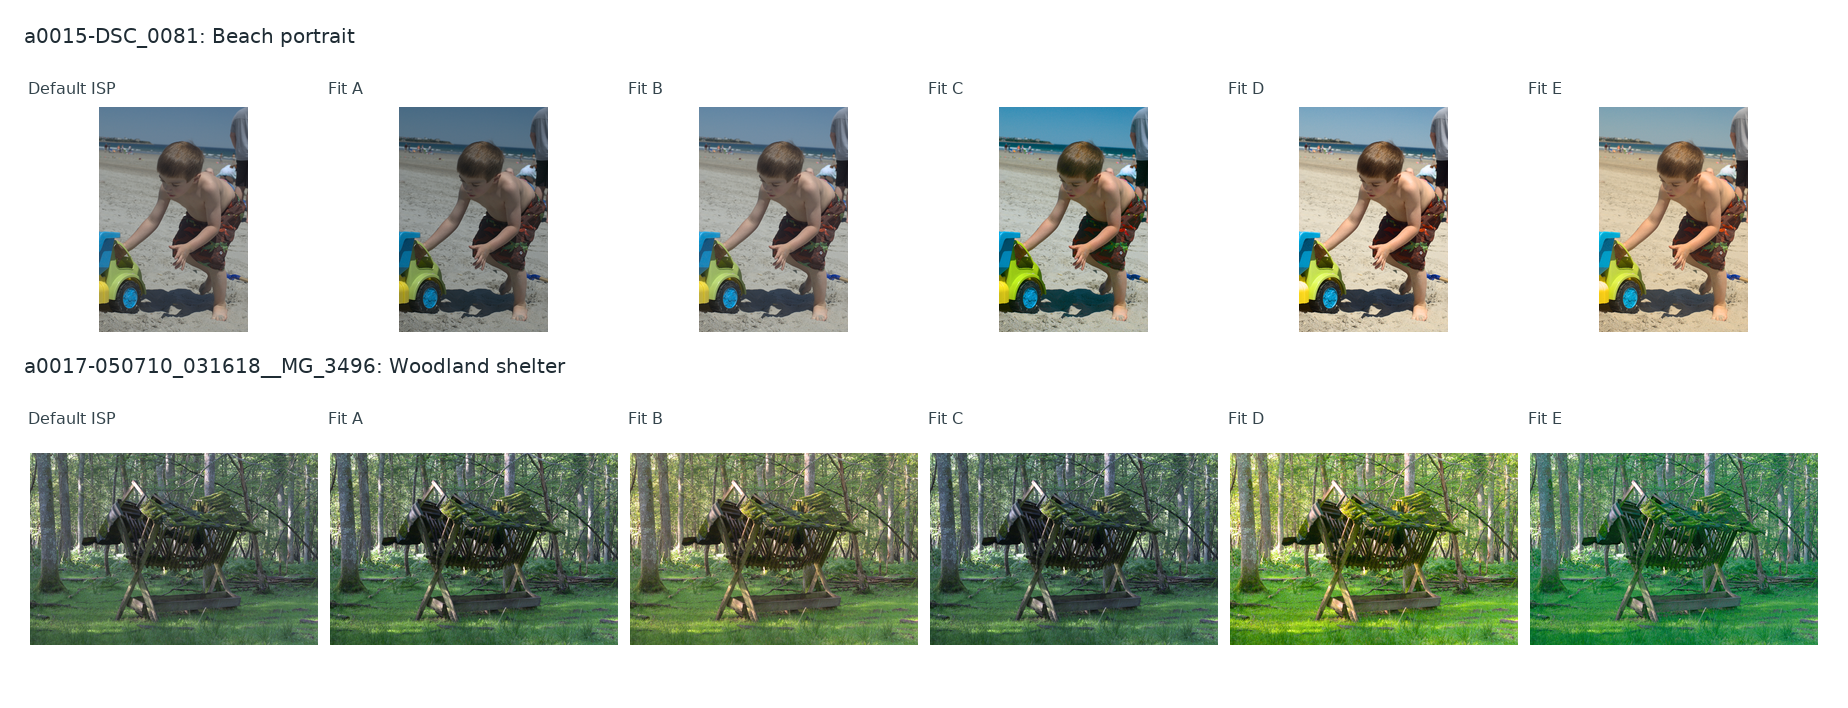
\includegraphics[width=\textwidth]{figures/fivek_fit_examples.png}
\caption{Default ISP and fitted ISP outputs for two FiveK-ISPVA-105 scenes. Each row shows Default ISP once followed by fitted outputs A--E. Example images are the saved 720-pixel-short-side renders; the expert TIFF is omitted here because the descriptions target fit versus Default ISP. The montage-generation script is listed in the Reproducibility section.}
\label{fig:fivek-fit-examples}
\end{figure*}

\begin{table}[t]
\caption{Example annotation and approximate style references for scene a0015-DSC\_0081, fit A.}
\label{tab:annotation-example}
\centering
\footnotesize
\begin{tabularx}{\columnwidth}{l X}
\toprule
Field & Stored annotation \\
\midrule
D1 & Cooler light keeps the beach subdued. \\
D2 & The boy and toy sit in a quiet, low-key summer frame. \\
D3 & Pale blue sea; shaded child and sand. \\
D4 & A restrained coastal-film look, with cool daylight and deep foreground shade. \\
Style name & Quiet Shore (assistant-authored) \\
App resemblance & Instagram Classic: Gingham; VSCO: A4 (approximate visual references) \\
\bottomrule
\end{tabularx}
\end{table}

The manifest \path{experiments/semantic_parameter_learning/fivek_isp_visual_annotation_dataset.json} records component files, scene coverage, resolution, provenance, and SHA-256 hashes. Source images and TIFF masters remain external; redistribution terms require separate verification.

For data maintenance, a consolidated FiveK-ISPVA release is assembled by \path{experiments/semantic_parameter_learning/package_fivek_dataset.py}. It merges the 105-scene experimental core and the completed 20-scene acquisition pilot, yielding 125 visually annotated scenes, 625 expert-fit pairs, and 2,500 D1-D4 descriptions, with no pending fit descriptions. The unified description document retains source and scene-level provenance; the original source documents remain separate for audit. These expanded collection counts do not change the 105-scene fitting results reported below. Each release preserves original RAW and expert TIFF masters, 720-pixel-high default/target/fit renders, all linguistic source documents and annotation provenance, physical and normalized fitting parameters, historical experiment archives, calibration records, a unified visual report, and expert-specific statistics. Full-resolution fitted outputs were not collected; reduced-resolution detail descriptions must not be presented as validated original-resolution sharpness labels. Immutable release manifests and checksums support auditing, while redistribution clearance remains a prerequisite for publication.

\section{Current Results: Exp81 and FiveK-ISPVA-105}
\subsection{Active Exp81 Endpoints}
Exp81 reuses 1,344 saved descriptor-image tuning records, computes one median per descriptor over seven images, and selects the directional q90 of the 16 medians per pole. The top two descriptors per pole also define the active centroid. Table~\ref{tab:endpoints} gives the selected physical endpoints; the negative endpoint is the numeric q10 and the positive endpoint the numeric q90. The settings are calibration outputs, not perceptual preference scores.

\begin{table*}[t]
\caption{Active CLIP Exp81 isolated physical pole settings. Inactive controls are neutral.}
\label{tab:endpoints}
\centering
\footnotesize
\begin{tabular}{lrr}
\toprule
Control & Negative pole & Positive pole \\
\midrule
Warmth & -0.262357 & +0.247906 \\
Saturation & -0.874711 & +0.862060 \\
Tone gain & 0.083463 & +3.757285 \\
Contrast & 0.249646 & +2.632414 \\
Sharpness & -0.805491 & +0.728980 \\
Palette coordinate & -0.198785 & +0.190551 \\
\bottomrule
\end{tabular}
\end{table*}

Each endpoint is a direction-aligned q90 across 16 descriptor medians, where each median pools seven image settings. Exp81's selected phrase centroids are coupled to this same descriptor tail. Tone-gain settings approach both legal extremes, illustrating the importance of explicit bounds. They are model- and descriptor-specific calibration settings, not a perceptual scale.

\subsection{FiveK Fit Statistics}
The 105-scene run contains 525 completed pairs (five photographer targets per scene), each optimized for 500 iterations. Mean in-sample display-sRGB MAE decreases from 0.1233 for Default ISP to 0.0321 for the fitted ISP; mean relative reduction is 70.2\%, with all 525 pairs below their own Default ISP baseline. This is the same-image fitting objective, not held-out performance, perceptual quality, or evidence that the six-control ISP reproduces local edits.

\subsection{Recent Calibration and Geometry Diagnostics}
Exp63--67 developed the nearest-swatch palette and moderated its strength after CLIP-only tuning favored stronger color; Exp68--71 compared color-protection choices and retained palette-only gray/skin protection. Exp70 compared CLIP and SigLIP with independent calibrations; Exp72 tested a curated 24-word subset on three scenes, which is not full-corpus generalization. Exp73 tested stronger v8 warmth, brightness, and saturation wording. The current v14/Exp81 pipeline supersedes that v8 setup by recomputing endpoints and centroids from selected descriptor tails.

Exp82 projects normalized 512-D CLIP descriptor embeddings and selected pole centroids into a two-dimensional metric-MDS plot. For warmth, the 204-point fit has normalized stress 0.329 and retains 52.8\% of the original 512-D negative-to-positive centroid distance; this is a lossy visualization, not a separability result. Exp83 fits a linear SVM to the 32 authored warmth descriptors: training accuracy is 32/32 and leave-one-phrase-out accuracy is 31/32 (one negative-pole D3 phrase is misclassified). These are diagnostics on authored phrases only, not tests of unseen words or images.

\section{Historical Calibration and Backbone Diagnostics (Exp63--Exp73)}
The following subsections report historical calibration stages and are not the active Exp81 configuration.
\subsection{Palette Calibration Ablation History}
Exp63 introduced the nearest-swatch operator with aggressive descriptors and full-endpoint directional prior; its endpoints were -0.323222/+0.332589. Exp64 averaged those saved settings, without rerunning the image optimizer, producing -0.296040/+0.303076. Exp65 swept 17 values over $[-0.4,+0.4]$ on three scenes; mean CLIP cosine peaked at +0.40 for teal-orange and -0.35 for magenta-green. These are same-model self-scores, not preference results. Exp66 used moderated descriptors, target 0.20, and prior weight 0.60, giving q90 settings -0.241714/+0.226108. Exp67 moved only the prior target to 0.17 and retained q90 selection, yielding the endpoints above.

\subsection{Side-by-Side Pole Renders and Evaluation Status}
The Exp70 index provides neutral/CLIP/SigLIP SBS pole sheets for scenes 2, 33, and 384 under combined color protection. Exp71 provides the final palette-only protection configs. These isolated pole renders are not free-text centroid requests.

Exp72 runs the final model-specific mappings on twelve clear control words (warm, cool, bright, dark, saturated, muted, sharp, monochrome, retro, golden, faded, crisp) and twelve subjective held-out words (angelic, ancient, ethereal, noir, tropical, gothic, melancholic, futuristic, pastoral, mystical, whimsical, bohemian), using the template ``a $w$ photo.'' On scenes 2, 33, and 384, the mean maximum-axis coordinate gap between models is 0.133 for easy and 0.089 for hard prompts; mean rendered RGB MAE is 6.89/255 and 6.58/255, respectively. The largest coordinate differences include faded on sharpness (+0.400 SigLIP minus CLIP), saturated on saturation (-0.240), muted on saturation (+0.222), and angelic on brightness (-0.207). Melancholic has the largest mean render difference (23.30/255). These are model-mapping and pixel-difference diagnostics, not quality or preference scores. The side-by-side sheets and mapping CSV are saved under \path{/data/data1/semantic_isp/results/exp72_backbone_inference_easy_hard/}.

This is a curated 24-prompt inference subset, not a full-corpus generalization evaluation. Earlier held-out and full-corpus CLIP scores belong to prior descriptor/calibration versions and are not reported as Exp71/Exp72 results. No human preference study, independent VLM evaluation, uncertainty analysis, or statistical significance test has been conducted.

\section{Discussion and Limitations}
The active evidence is an engineering calibration, not evidence that the six semantic axes are perceptually independent or that the selected endpoints are preferred. Exp81's selected centroid descriptors are part of the descriptor set used for endpoint ranking; they are not an independent holdout. The FiveK optimized fit results are in-sample, and the annotation text is subjective assistant-authored material, not human consensus or ground truth. The model name GPT-5.6 Luna is reported from a screenshot of a verification execution and cannot be attributed conclusively to the original annotation turns.

Coverage also differs by annotation component: fitted-render D1-D4 prose covers 105 scenes / 525 fits, whereas filter-style labels, approximate Instagram/app resemblance references, and the separate expert-versus-default prompts cover 11 scenes / 55 fits each. The app references are subjective look analogies, not exact filter simulations. Descriptions were written from reduced-resolution comparison sheets with Expert TIFFs visible as context; sharpness was not assessed from full-resolution crops. No user/colorist ratings, inter-rater agreement, independent VLM validation, uncertainty analysis, full-corpus final-config evaluation, temporal test, hardware/runtime/power measurement, or camera transfer study exists. RAW/TIFF assets and model weights remain external, and redistribution terms require verification.

\section{Conclusion}
This paper documents the active Exp81 six-DOF semantic ISP, descriptor-median direction-aligned q90 endpoints, two-phrase CLIP centroids, and FiveK-ISPVA-105, a 105-scene dataset with 525 fitted renders and 2,100 D1-D4 descriptions. The style-name and Instagram/app-reference component remains limited to 11 scenes. The optimization results are calibration and in-sample fit evidence only. Independent human evaluation, full-resolution visual review, and broader request-level testing remain necessary before making preference, professional-validity, or open-vocabulary claims.

\appendices
\section{Selected Exp81 Pole Phrases}
\begin{table*}[t]
\caption{The two selected descriptors per pole used to form active Exp81 CLIP text centroids. Each pole has 16 total descriptors; the complete banks are in the machine-readable descriptor file.}
\label{tab:selected-phrases}
\centering
\footnotesize
\begin{tabularx}{\textwidth}{l X X}
\toprule
Pole & Selected phrase 1 & Selected phrase 2 \\
\midrule
Warmth, negative & Overwhelmingly cold sterile fluorescent atmosphere & Strong icy-blue shift in highlights and midtones \\
Warmth, positive & Extreme sunset-orange film grade & Overheated golden-hour color wash \\
Saturation, negative & Restrained monochrome art house atmosphere & Faded monochrome archival print \\
Saturation, positive & Explosive neon festival colors & Brilliant oversaturated hues across the entire photograph \\
Brightness, negative & Near-complete darkness swallowing the entire image & An extremely dark, almost pitch-black scene \\
Brightness, positive & Intensely luminous and overwhelmingly bright appearance & Blazing, severely overexposed summer daylight \\
Contrast, negative & Low contrast vintage matte print & Quiet flat tonal softness \\
Contrast, positive & Dramatic high-contrast noir with crushed shadows and brilliant whites & Striking graphic contrast separating dark shadows from bright light \\
Sharpness, negative & Heavy Gaussian blur across the entire photograph & Deeply blurred indistinct dreamlike scene \\
Sharpness, positive & Hyperreal oversharpened digital photograph & Razor-sharp outlines with ringing edge halos \\
Palette, negative & Stylized magenta-green photographic palette & Complementary magenta-green photographic color grading \\
Palette, positive & Stylized warm orange and ocean teal & Cinematic teal-orange color grade \\
\bottomrule
\end{tabularx}
\end{table*}

\section{Reproducibility}
The active method and file map are \path{experiments/semantic_isp/CURRENT_METHOD.json} and \path{experiments/semantic_isp/README.md}. Exp81 aggregation is implemented in \path{experiments/semantic_isp/exp81_descriptor_tail_calibration.py} and can be rebuilt from the saved Exp80 phrase-image records with:
\begin{quote}\footnotesize\ttfamily
python experiments/semantic\_isp/exp81\_descriptor\_tail\_calibration.py --base /data/data1/semantic\_isp/results/exp80\_v14\_additive\_contrast/contrast --out /path/to/new\_exp81 --images 2 33 384 --device cuda:0
\end{quote}
Projection and rendering are in \path{experiments/semantic_isp/moran_semantic_isp.py} and \path{experiments/semantic_isp/axis_isp.py}. The 105-scene FiveK fit uses \path{experiments/semantic_parameter_learning/fivek_photographer_fit.py} with 500 iterations, learning rate 0.03, and scene IDs recorded in the source run's \path{index.json}; the report renderer is \path{experiments/semantic_parameter_learning/fivek_screen_comparisons.py}. The named dataset manifest is \path{experiments/semantic_parameter_learning/fivek_isp_visual_annotation_dataset.json}; the figure in Fig.~\ref{fig:fivek-fit-examples} is reproducible with \path{experiments/semantic_parameter_learning/render_tip_fit_examples.py}. Before submission, verify references and author details, establish redistribution terms, and add independent request-level and human evaluation.

\begin{thebibliography}{99}
\bibitem{radford2021clip}
A. Radford \emph{et al.}, ``Learning transferable visual models from natural language supervision,'' in \emph{Proc. Int. Conf. Mach. Learn.}, 2021, pp. 8748--8763.
\bibitem{zhai2023siglip}
X. Zhai \emph{et al.}, ``Sigmoid loss for language image pre-training,'' in \emph{Proc. IEEE/CVF Int. Conf. Comput. Vis.}, 2023.
\bibitem{lee2024cliptone}
H. Lee, K. Kang, J. Ok, and S. Cho, ``CLIPtone: Unsupervised learning for text-based image tone adjustment,'' in \emph{Proc. IEEE/CVF Conf. Comput. Vis. Pattern Recognit.}, 2024, pp. 2942--2951.
\bibitem{mayer2025language}
O. Mayer, S. Noguchi, A. Berestov, and J. Takatori, ``Language-based color ISP tuning,'' in \emph{Proc. IS\&T Color Imag. Conf.}, 2025, pp. 203--208; arXiv:2509.10765.
\bibitem{shi2021t2onet}
J. Shi, N. Xu, and others, ``Learning by planning: Language-guided global image editing,'' in \emph{Proc. IEEE/CVF Conf. Comput. Vis. Pattern Recognit.}, 2021.
\bibitem{kimlee2024crisp}
H. Kim and K. M. Lee, ``Learning controllable ISP for image enhancement,'' \emph{IEEE Trans. Image Process.}, vol. 33, 2024, pp. 867--880.
\bibitem{yoshimura2023dynamicisp}
M. Yoshimura, J. Otsuka, A. Irie, and T. Ohashi, ``DynamicISP: Dynamically controlled image signal processor for image recognition,'' in \emph{Proc. IEEE/CVF Int. Conf. Comput. Vis.}, 2023.
\bibitem{wang2023clipiqa}
J. Wang, K. C. K. Chan, and C. C. Loy, ``Exploring CLIP for assessing the look and feel of images,'' in \emph{Proc. AAAI Conf. Artif. Intell.}, 2023.
\bibitem{bychkovsky2011fivek}
V. Bychkovsky, S. Paris, E. Chan, and F. Durand, ``Learning photographic global tonal adjustment with a database of input/output image pairs,'' in \emph{Proc. IEEE Conf. Comput. Vis. Pattern Recognit.}, 2011, pp. 97--104.
\end{thebibliography}

\end{document}
